\documentclass[compress,11pt]{beamer}
%\includeonly{pendel}
\usetheme{Ilmenau}
%\usetheme{fau-4-3}
%\usecolortheme{beaver}
\beamertemplatenavigationsymbolsempty
\usepackage[ngerman]{babel}
\usepackage{marvosym}
\usepackage{multimedia}
\usepackage[utf8]{inputenc}
\usepackage{amsmath}
\usepackage{amsfonts}
\usepackage{amssymb}
\usepackage{graphicx}
\usepackage{esvect}
%\author{}
\title{EP Gruppe 8}
%\setbeamercovered{transparent}
%\setbeamertemplate{navigation symbols}{}
%\logo{}
%\institute{}
%\date{}
%\subject{}
\usepackage{verbatim}
\begin{document}
\begin{frame}
\begin{block}{Eigenschaften eines Dehnungsstreifens}
\begin{itemize}
\item Leiter, die bei geringsten Verformungen ihren Widerstand verändern
\item werden normalerweise in dünne Folien eingefertigt
\item Relative Widerstandsänderung ergibt sich durch $\frac{\Delta R}{R} + \frac{\Delta \rho}{\rho} + \frac{\Delta l}{l} - \frac{2 \cdot \Delta D}{D}$
\end{itemize}
\end{block}

Es wurde der Widerstand eines Dehnungsmessstreifens unter Belastung durch verschiedene Gewichte gemessen, um eine Kalibrierkurve zu erstellen. Die Masse des mit "???" gekennzeichneten Blocks war zu ermitteln\\
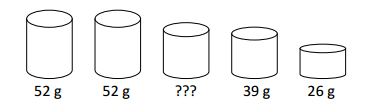
\includegraphics[width=.5\textwidth]{../massen}

\end{frame}
\begin{frame}
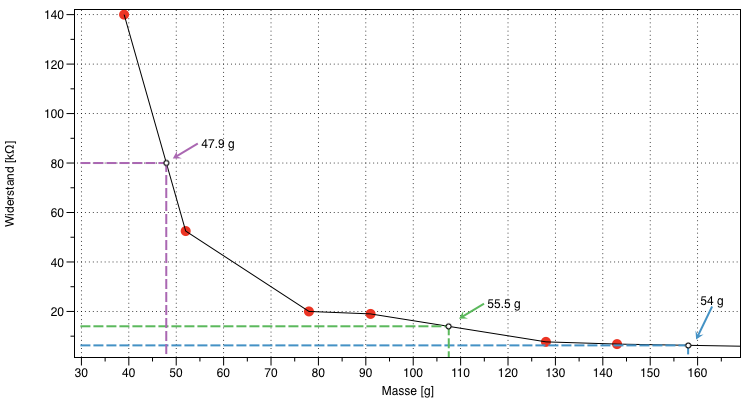
\includegraphics[width=.7\textwidth]{../dehnungsstreifen}\\
Durch lineares Interpolieren zwischen zwei Mess-Punkten mit bekannten Massen erhält man als Mittelwert aus drei verschiedenen Massekombinationen einen Mittelwert von $m \approx 52.5 g$
\end{frame}
\begin{frame}
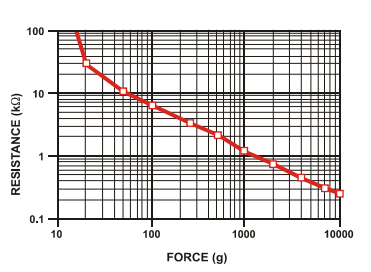
\includegraphics[width=.4\textwidth]{../datenblatt_kurve}
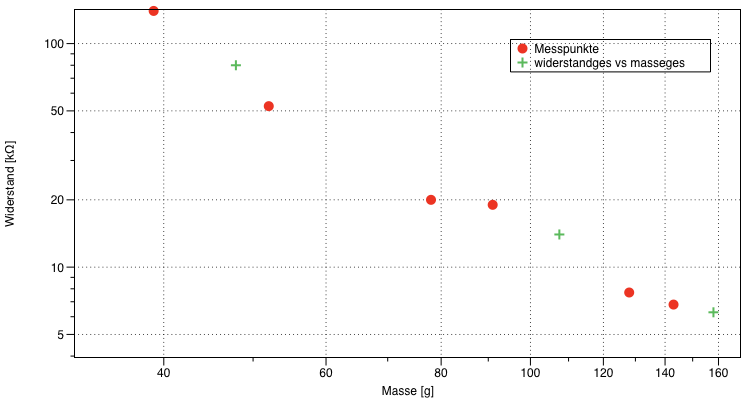
\includegraphics[width=.5\textwidth]{../dehnungsstreifenlog}\\
Grober Vergleich der gemessenen Kalibrierungskurve (rechts) mit der aus dem Datenblatt
\end{frame}
\end{document}